\section{Formální definice kryptografického systému, symetrické a asymetrické šifry. Výpočetně těžké matematické problémy pro~asymetrické šifry.}

\subsection{Definice}

\uline{Kryptografický systém} pro~šifrování zpráv je pětice $(\mathcal{M}, \mathcal{C}, \mathcal{K}, \mathcal{E}, \mathcal{D})$, kde
$\mathcal{M}$ je prostor otevřených zpráv,
$\mathcal{C}$ prostor šifrových zpráv,
$\mathcal{K}$ prostor klíčů,
$\mathcal{E}, \mathcal{D}$ dvojice zobrazení, které každému klíči $k \in \mathcal{K}$ přiřazují transformaci pro~zašifrování zpráv $E$ a~transformaci pro~dešifrování zpráv $D$, kde platí $D(k(E(k,m))=m \ \forall \ k \in \mathcal{K}, m \in \mathcal{M}$.

\uline{Symetrická šifra} je taková šifra, kde pro~každé $k \in \mathcal{K}$ lze z~transformace zašifrování $E_k$ určit transformaci dešifrování $D_k$ a naopak.

\uline{Asymetrická šifra} je taková šifra, kde pro~skoro všechna $k \in \mathcal{K}$ nelze z~transformace pro~zašifrování $E_k$ určit transformaci dešifrování $D_k$.
Bývá zde přítomen tajný klíč $k$, ze~kterého se vhodnou transformací $G$ vygeneruje dvojice parametrů $(e, d)$, která tvoří veřejné a~privátní klíče ($k_\text{pub}$, $k_\text{priv}$).
Ty parametrizují transformace šifrování a dešifrování.

\subsection{Matematické problémy asymetrických šifer}

\subsubsection{Problém diskrétního logaritmu}

Rovnice $c \equiv m^n \mod p$ je výpočetně jednoduchá a rychlá, získání $m$ z~$c$ je naopak složité.

DLP využívají protokoly Diffie-Hellman, ElGamal, DSA, ECDL, ECDSA, \dots

Mezi algoritmy řešení patří brute-force, baby step--giant step, Pollardův $\rho$ algoritmus, funkční síto, \dots

\subsubsection{Problém faktorizace}

Faktorizace je proces převodu složeného čísla na~jeho prvočíselné složky.

FP využívá například RSA.

Mezi algoritmy řešení patří brute-force, Pollardůvo $\rho$ algoritmus, Pollardův $\rho - 1$ algoritmus, Lehmannova metoda, kvadratické síto, \dots


\clearpage
\section{Služby bezpečnosti zajišťované kryptografickými prostředky, kryptografické mechanismy, které tyto služby zajišťují.}

\subsection{Služby}

\uline{Autentizace} (\emph{authentication}) je proces ověření identity entity.
\emph{Peer Entity Authentication} ověřuje uživatele,
\emph{Data Origin Authentication} ověřuje všechna data a eliminuje např. útoky opakováním.

\uline{Řízení přístupu} (\emph{access control}) je možnost povolit či odepřít použití určitého zdroje určitému subjektu.

\uline{Zabezpečení důvěrnosti dat} (\emph{data confidentiality}) je ochrana obsahu proti analýze.
Může jít o~zajištění důvěrnosti přenosu zpráv, spojení, toku dat nebo služby selektivní důvěrnosti (které chrání pouze část informace).

\uline{Zabezpečení integrity dat} (\emph{data integrity}) je ochrana proti neautorizované modifikaci.
Slabá integrita: modifikace zprávy šumem, změna pořadí paketů, náhodná duplicita (kontrolní součet, CRC, pořadové číslo).
Silná integrita: podvržení zprávy, úmyslné pozměnění zprávy; bez~oprav a s~opravami.

\uline{Ochrana proti odmítnutí původu zprávy} (\emph{non-repudiation}) zajišťuje důkaz o~původu dat a dokazuje původ nebo doručení.

\subsection{Mechanismy}

Šifrování, digitální podpisy, řízení přístupu, mechanismy integrity dat, výměna autentizační informace, padding, řízení směrování, ověření třetí stranou.

\begin{table}[ht]
	\centering
	\onehalfspacing

	\begin{tabular}{|l|cccccccc|}
		&
		\begin{sideways}šifrování\end{sideways} &
		\begin{sideways}podpis\end{sideways} &
		\begin{sideways}řízení přístupu\end{sideways} &
		\begin{sideways}integrita\end{sideways} &
		\begin{sideways}autentizace\end{sideways} &
		\begin{sideways}padding\end{sideways} &
		\begin{sideways}řízení směrování\end{sideways} &
		\begin{sideways}ověření třetí stranou\end{sideways} \\
		\hline\hline
		%                              š   p   ř   i   a   p   ř   o
		autentizace spojení          & X & X &   &   & X &   &   &   \\
		autentizace odesílatele      & X & X &   &   &   &   &   &   \\
		řízení přístupu              &   &   & X &   &   &   &   &   \\
		důvěrnost spojení            & X &   &   &   &   &   &   &   \\
		důvěrnost přenosu zpráv      & X &   &   &   &   &   & X &   \\
		selektivní důvěrnost         & X &   &   &   &   &   & X &   \\
		důvěrnost toku dat           & X &   &   &   &   & X & X &   \\
		integrita spojení s~opravou  & X &   &   & X &   &   &   &   \\
		integrita spojení bez~opravy & X &   &   & X &   &   &   &   \\
		selektivní integrita spojení & X & X &   & X &   &   &   &   \\
		integrita přenosu zpráv      & X & X &   & X &   &   &   &   \\
		nepopiratelnost odesílatele  & X & X &   & X &   &   &   & X \\
		nepopiratelnost doručení     & X & X &   & X &   &   &   & X \\
	\end{tabular}

	\caption{Matice mechanismů bezpečnosti}
\end{table}


\clearpage
\section{Kryptograficky bezpečné generátory náhodných čísel –- požadavky, hodnocení bezpečnosti, příklady realizace.}
\subsection{Požadavky}
\begin{itemize}
    \item \uline{Next-bit test} -- je-li známo prvních $k$ bitů náhodné posloupnosti, neexistuje žádný algoritmus s~polynomiální složitostí, který by dokázal předpovědět $(k + 1)$ bit s~pravděpodobností vyšší než 1/2.
    \item \uline{State compromise} -- i~když je zjištěn vnitřní stav generátoru (celý nebo z~části), nelze zpětně zrekonstruovat dosavadní vygenerovanou posloupnost. Navíc, pokud do~generátoru za~běhu vstupuje další entrope, nemělo by být možné ze~znalosti vnitřního stavu předpovědět vnitřní stav v~následujících iteracích
    \item vetšina používaných PRNG tyto požadavky splňuje jen za~určitých podmínek
\end{itemize}

\subsection{Hodnocení bezpečnosti}
Entropie
\begin{itemize}
    \item veličina entropie popisuje míru náhodnosti -- jak obtížné je hodnotu (náhodné číslo, náhodnou posloupnost, řetězec náhodných bitů) uhodnout
    \item míra nejistoty (nepředvídatelnosti) hodnoty a závisí na~pravděpodobnostech možných výsledků procesu, který ji generuje
    \item dána vztahem:
\end{itemize}
\begin{align*}
    H(X) = - \displaystyle\sum\limits_{i-1}^n p_{i} \log_2 p_{i} 
\end{align*}
\begin{itemize}
    \item X - generovaná hodnota
    \item $p_{1},..., p_{n}$ - pravděpodobnosti všech hodnot $X_{1},..., X_{n}$, které je daný generátor schopen vygenerovat
    \item vztahuje se k~útočníkovu a jeho schopnosti předpovídat vygenerovanou hodnotu -- pokud útočník následující generovanou hodnotu s~jistotou zná, entropie je nulová = nulová bezpečnosti aplikace, která takto vygenerovanou náhodnou hodnotu využívá
    \item vyjadřuje průměrný počet bitů nutných k~zakódování hodnoty při~použití optimálního kódování
    \item vyjadřuje obsažené množství informace vyjádřené v~bitech
    \item entropie generátoru je maximální, pokud se pro~danou délku (počet bitů) generují všechny možné posloupnosti, každá z~nich se stejnou pravděpodobností
\end{itemize}

\subsection{Příklady realizace}
Generátor pseudonáhodných čísel (PRNG)
\begin{itemize}
    \item algoritmicky řešení generátory, využívají výpočetních / SW metod
    \item základní problém -- jakýkoliv v současnosti existující program je deterministický = existuje pouze jedna možnost, jak k~výsledku dojít
    \item možnost se může jevit náhodná, ale není
    \item pro~člověka pouze není snadné zjistit, jakým způsobem byla vytvořena
    \item výhody: rychlé, snadno realizovatelné, lze nastavit odchylku rozložení
    \item nevýhody: malá bezpečnost, periodicita
\end{itemize}

Kryptograficky bezpečené PRNG
\begin{itemize}
    \item pokud PRNG splňuje určité požadavky $\rightarrow$ považujeme na~kryptograficky bezpečné
    \item vyžadují náhodný a tajný vstup (\emph{seed}) -- nelze se tedy obejít bez \enquote{skutečné náhody}
    \item kvalita závisí na~kvalitě generování hodnoty \emph{seed}
    \item entropie výstupu PRNG je dána entropií, která vstupuje (\emph{seed}), algoritmus samotný nikdy nemůže entropii zvyšovat
    \item zdroj entropie např.: sběr událostí z~pohybu myši, klávesnice, HD a některých přerušení (Linux PRNG)
    \item podmínky:
    \begin{itemize}
        \item Next-bit test
        \item State compromise
    \end{itemize}
    \item příklady:
    \begin{itemize}
        \item bloková šifra v~režimu čítače -- náhodně se zvolí klíč / seed a počáteční hodnota čítače $i$. Zvoleným klíčem se postupně šifrují hodnoty $i$, $i+1$, atd. dokud nedojde k~překročení velikosti bloku -- perioda
        \item hashovací funkce aplikovaná na~čítač -- náhodně se zvolí počáteční hodnota čítače $i$. Postupně se hashují hodnoty $i$, $i+1$ atd. Nesmí dojít k prozrazení počáteční hodnoty čítače
        \item proudové šifry -- v~zásadě PRNG, s~jehož výstupem se provádí XOR s~otevřeným textem
        \item algoritmy založené na~teorii čísel -- u~kterých byl proveden důkaz bezpečnosti
    \end{itemize}
\end{itemize}

Generátory skutečně náhodných čísel (TRNG)
\begin{itemize}
    \item využívající fyzikální / HW metody
    \item zdroj entropie -- klasický nebo kvantový fyzikální jev
    \item výhody: vysoká bezpečnost, neopakovatelnost
    \item nevýhody: pomalé, problémy s~realizací, ne vždy lze dosáhnout maximálně rovnoměrného rozložení
\end{itemize}



\clearpage
\section{Hašovací funkce, formální definice, požadované vlastnosti, hodnocení bezpečnosti, příklady algoritmů a použití.}

\begin{itemize}
    \item hašovací funkce je matematická funkce (resp. algoritmus) pro~převod vstupních dat do~malého čísla
    \item formálně jde o~funkci $h$, která převádí vstupní posloupnost bitů na~posloupnost pevné délky $n$ bitů
    \item použití:
    \begin{itemize}
        \item tvorba digitálních podpisů -- otisky zprávy
        \item kontrola integrity, porovnání souborů -- otisk souboru
        \item jednoznačná identifikace dat
        \item uložení hesel -- otisky hesel
        \item uložení klíčů -- otisky klíčů
        \item prokazování autorství
        \item pseudonáhodné generátory
    \end{itemize}
\end{itemize}

\subsection{Požadavky}
\begin{itemize}
    \item k~\enquote{libovolně} velkému vstupu $M$ -- pevná délka výstupu $h$
    \item jednocestnost (one-way)
    \begin{itemize}
        \item pro~danou zprávu $M$ lze snadno spočítat $h = h(M)$
        \item je-li dáno $h$, je velmi těžké spočítat $M$, ne však nemožné
    \end{itemize}
    \item bezkoliznost (collision-free)
    \begin{itemize}
        \item je velmi těžké nalézt různá $M$ a $M'$ tak, aby $h(M) = h(M')$
    \end{itemize}
\end{itemize}

Odolnost proti kolizím
\begin{itemize}
    \item kolize zákonitě existují, ale je oblížné je nalézt
\end{itemize}
\begin{enumerate}
    \item kolize prvního řádu (preimage resistance)
    \begin{itemize}
        \item nalezení vzoru
    \end{itemize}
    \item kolize druhého řádu (second preimage resistance)
    \begin{itemize}
        \item k dané zprávě $M_{1}$ nalézt zprávu $M_{2}$ tak, aby platilo $h(M_{1}) = h(M_{2})$
    \end{itemize}
    \item odolnost vůči kolizím (collistion resistance)
    \begin{itemize}
        \item nalezení dvou libovolných zpráv $M$ a $M'$, pro které platí $h(M) = h(M')$
    \end{itemize}
\end{enumerate}

\subsection{Hodnocení bezpečnosti}
Útoky, cílem je nalezení kolize
\begin{itemize}
    \item hrubou silou -- metoda totálních zkoušek -- závisí na~délce hašovacího kódu
    \item kryptoanalýzou -- zaměřená především na vnitřní strukturu haš. fce, především na~kompresní funkci $f$
\end{itemize}

\subsection{Princip konstrukce - iterační}
\begin{itemize}
    \item tento princip používají drtivá většina dnes používaných hashovacích funkcí
    \item algoritmus je založený na opakovaném použití kompresní funkce $f$ (= je jádrem hashovacích funkcí)
    \item proces iteračního výpočtu hashového kódu $h$ je možné vyjádřit v~následujícím tvaru:
\end{itemize}
\begin{align*}
    IV &= h_{0} \\
    h_{i} &= f (h_{i-1}, M_{i}), pro 1 \leq i \leq n \\
    h &= h_{n} \\
\end{align*}
\begin{itemize}
    \item tzn. kompresní funkce má dva vstupy a jeden výstup
    \item ypracovává aktuální blok zprávy $M_{i}$ a hodnotu $h_{i-1}$
    \item Výstupem je určitá hodnota $h_{i-1}$ (= kontext) $\longrightarrow$ ten pak použit jako vstup do kompresní funkce v dalším kroku
    \item počáteční hodnota kontextu $h_{0}$ - inicializační vektor IV - určuje blok bitů vstupující do první kompresní funkce a zahajuje tak vlastní hashování
\end{itemize}

\subsection{Pricip konstrukce - houba (SHA3)}
\begin{itemize}
    \item kryptografické primitivum využívající se v~mnoha aplikacích
    \item dvě fáze: absorpce a vymačkávání
    \item původní zpráva se po~bitech absorbuje v~první části pomocí kompresních funkcí $f$
    \item následně je vymačkávána tolikrát, dokud nemáme odpovídající velikost výstupu
    \item příklady: SHA-3 (algoritmus Keccak)
    \begin{itemize}
        \item SHA-3 hash -- digitální podpis, integrita dat, identifikace dat
        \item SHA-3 MGF -- generování klíčů, hashování v~PKI
        \item SHA-3 solená hash -- ukládání hesel
        \item SHA-3 MAC -- jednodušší než HMAC
        \item SHA-3 proudová šifra
    \end{itemize}
\end{itemize}


\clearpage
\section{Kryptografie nad eliptickými křivkami, principy, důvody použití, příklady algoritmů.}


\clearpage
\section{Digitální podpis, principy, standardy, metody pro distribuci veřejných klíčů (PKI).}


\clearpage
\section{Kvantová distribuce klíčů, důvody použití, příklady protokolů.}

QKD (\emph{Quantum Key Distribution}) používá pro~komunikaci kvantové jevy, např. spin fotonu.

Z~důvodu Heisenbergova principu neurčitosti není možné vytvořit kopii neznámého kvantového stavu: čtení zprávy ovlivňuje její obsah.

Qubit může nabývat libovolné hodnoty z~intervalu $\left<0,1\right>$, ale měřením lze získat nejvýše jeden bit klasické informace.
Qubity mohou být realizovány jakýmkoliv dvojrozměrným kvantovým systémem: foton (polarizace, fázový posun), elektron (spin), atom (spin).


\subsection{Důvody použití}

Protokoly distribuce klíčů postavené na~klasické kryptografii (např. DH) jsou kvantově zlomitelné.
QKD staví bezpečnost na~fyzikálních principech které není možné kvantově obejít.

Foton nelze rozdělit a ani není možné vytvořit jeho přesnou kopii.
Eva, stojící mezi Alicí a Bobem, nezná polarizační bázi, a v~přenosu tedy způsobí přibližně 50\,\% chyb.
Stálý odposlech tedy způsobí přibližně 25\% chybovost.


\subsection{QKD protokoly}

\begin{table}[ht]
\subsubsection*{BB84}
\centering
\onehalfspacing
\begin{tabular}{lll}
Alice & \verb@1111100101000010000100000@ & výběr zprávy \\
      & \verb@x+xxxxx+xx++++xx++x++xx++@ & polarizace náhodnou bází \\
      & \verb@/-///\\-\/||||/\||\-|\\||@ & přenositelná zpráva ve~čtyřech možných orientacích \\
Bob   & \verb@++x+xx+x+x++xx+xx+x+x+++x@ & dekódování qubitů v~náhodných bázích \\
      & \verb@ 111100 11000 000001 1 01@ & (některé bity byly ztraceny při~přenosu) \\
\hline
Bob   & \verb@ +x+xx+ +x++x +xx+x+ + +x@ & poslání bází Alici \\
Alice & \verb@ .. ..   ...   . ...   . @ & potvrzení správně vybraných bází \\
      & \verb@ 11 10   100   0 001   0 @ & \dots je materiál klíče \\
\hline
      & \verb@    10   10    0 00    0 @ & \dots je klíč po~obětování bitů \\
\end{tabular}
\caption{
Bity 0, 1 jsou kódovány do~kvantových stavů polarizovaných fotonů.
Jde o~dvě navzájem kolmé lineární polarizace ve~dvou bázích vůči sobě otočených o~45\textdegree. \\
\texttt{+|} $\rightarrow$ 0, \texttt{+-} $\rightarrow$ 1; \texttt{x\textbackslash} $\rightarrow$ 0, \texttt{x/} $\rightarrow$ 1}
\end{table}
\FloatBarrier

\begin{table}[ht]
\subsubsection*{B92}
\centering
\onehalfspacing
\begin{tabular}{lll}
Alice & \verb@0100101111010100010001110@ & výběr zprávy \\
      & \verb@-/--/-////-/-/---/---///-@ & polarizace náhodnou bází \\
Bob   & \verb@xx+++x+x++xx+xx+xx++xx++x@ & náhodné zvolení bází \\
      & \verb@\/--|/|/ -\/- /-\/--//-|/@ & polarizace přijatých bází \\
      & \verb@0???1?1? ?0?? ??0??????1?@ & \dots přijatý výsledek \\
\hline
Bob   & \verb@.   . .   .     .      . @ & poslání pozic dekódovaných quibitů \\
      & \verb@    1           0        @ & obětování bitů odesláním \\
Alice & \verb@    .           .        @ & potvrzení správnosti \\
\hline
      & \verb@0     1    0    0      1 @ & \dots je klíč \\
\end{tabular}
\caption{
Alice si vybírá jednu polarizaci v~každé bázi; jedna báze reprezentuje~0, druhá~1. \\
\texttt{-} $\rightarrow$ 0; \texttt{/} $\rightarrow$ 1}
\end{table}
\FloatBarrier

\subsubsection*{Šestistavový protokol}

Vychází z~BB84, ale používá polarizaci v~šesti směrech (\enquote{plus}, \enquote{kříž}, rotatce).

Všechny obětují část dohodnutého klíče a veřejným kanálem se informují o~přijatých hodnotách.
Tuto komunikaci je nutné autentizovat.
Při~obětování $n$ bitů je pravděpodobnost detekce soustavného odposlechu $1 - \left(\frac{1}{4}\right)^n$.

\subsubsection*{EPR}

Využívá kvantově provázaný pár fotonů.

\subsubsection*{\emph{Coherent One Way} (COW) protokol}

Bity kóduje do~koherentních pulzů.
Koherence se při~odposlechu i~přenosu velmi lehce naruší, na~což reaguje detektor.

Neexistuje obecný důkaz bezpečnosti COW.


\clearpage
\section{Postkvantová kryptografie -- důvody použití, jaké těžké matematické problémy se zde využívají (kryptosystém McEliece, kryptosystém založený na mřížkách). Jednorázový podpis pomocí hašovacích funkcí (Lamport).}

PQC (\emph{Post-Quantum Cryptography}) využívá matematické problémy které kvantové počítače nezvládají řešit o~nic rychleji než klasické.

DH (Diffie-Hellman), DLP (problém diskrétního logaritmu), FP (problém faktorizace), ECC (kryptografie nad~eliptickými křivkami) jsou kvantově řešitelné v~polynomiálních či polylogaritmických časech.
Pomocí Shorova (kvantová faktorizace), Groverova (kvantové prohledávání) a dalších algoritmů aplikovaných na~reálném kvantovém hardware se současná asymetrická kryptografie stává nedostatečně bezpečnou.

Mezi problémy postkvantově bezpečné patří například:

\begin{itemize}
\item mřížky (\emph{lattices}): matice o~mnoha dimenzích určující vektorovu mřížku,
\item polynomiální rovnice (\emph{multivariate equations}),
\item systémy založené na~hashích (\emph{hash-based systems}),
\item systémy založené na~kódech (\emph{code-based systems}): systémy postavené nad~protichybovým kódováním,
\item \emph{supersingular elliptic curve isogenies}: křivka ($k_\text{pub}$) a její morfismus na~jinou ($k_\text{priv}$).
\end{itemize}


\subsection{Mřížky}

Mřížka je množina bodů v~$n$-dimenzionálním prostoru v~periodické struktuře.
V~2D ji lze pomocí kartézských souřadnic $(x, y)$ definovat jako
$\mathcal{L} = \mathcal{L}(b_1, b_2) = \{x_i b_1 + x_i b_2 : x_i \in \mathbb{Z}\}$.

$n$-dimenzionální mřížka $\mathcal{L}$ je množina všech celočíselných kombinací $n$-lineárně nezávislých vektorů (generátorů) $b_1, \dots, b_n \in \mathbb{R}^n$:
$\mathcal{L} = \left\{ \sum_{i=1}^n x_i b_i : x_i \in \mathbb{Z} \right\}$.
$\mathcal{B} = \{b_1, \dots, b_n\}$ se nazývá Báze mřížky.
Při~bázi $\mathcal{B}$ mřížky $\mathcal{L}$ je každý vektor $v \in L$ vyjádřitelný jako unikátní lineární kombinace bázových vektorů, tj. $v = a_1 b_1 + \dots + a_n b_n$.

Obtížnost je obecně definována jako složitost nalezení dobré mřížky (tj. ortogonální) z~mřížky špatné (tvořené vektory s~umělými chybami).
Dobrá mřížka je soukromý klíč, špatná mřížka veřejný.

V~mřížkách jsou definovány problémy nejkratšího a nejbližšího vektoru.
SVP (\emph{Shortest Vector Problem}): Nejkratší vektor se v~neortogonální bázi hledá obtížně.
CVP (\emph{Closest Vector Problem}): Vektor nejbližší k~bodu mimo mřížku se hledá obtížně.
Oba jsou prokazatelně NP-těžké.

Mřížky se používají buď s chybami (\emph{Learning with Errors}), R-LWE (\emph{Ring-LWE}), M-LWE (\emph{Module-LWE}) nebo se~zaokrouhlováním (\emph{LWR}).
Jejich využití je především v~asymetrickém šifrování, výměně klíčů, digitálních podpisech, homomorfním šifrování nebo v~důkazech nulových znalostí.

Mezi praktické příklady patří kryptosystémy GGH (Enc, Sig), Dilithium (Sig), Kyber, Saber (KEM).


\subsection{McEliece}

Jde o~asymetrický systém $[n;k;t]$ postavený nad~protichybovým kódováním (\emph{binary Goppa code}) s~NP-těžkou obtížností.
Tvoří se náhodnou binární regulární maticí $\textbf{S}_{k \times k}$, generující maticí $\textbf{G}_{k \times n}$, náhodnou permutační maticí $\textbf{P}_{n \times n}$ a výslednou maticí $\textbf{G'}_{k \times n} = \textbf{SGP}$.
Veřejným klíčem je $[\textbf{G'}, t]$, soukromým $[S, G, P]$.

(Pravděpodobnostní) šifrování: $c = m\textbf{G'} + z$; (deterministické) dešifrování: $m' = D(c\textbf{P}^{-1})\textbf{S}^{-1}$ (kde $D$ je dekódovací algoritmus).
Privátním klíčem je~dekódovací algoritmus.
Proti RSA jde o~systém rychlejší, ale k~praktickému využití vyžaduje výrazně větší klíče ($| k_\text{pub} | \geq$ 512~Kb; resp. $\geq$ 6~Mb--8~Mb pro~postkvantovou bezpečnost).


\subsection{Lamport One Time Signature}

V~principu jde o~podepisování jednoho bitu $[0,1]$.
Jsou vygenerovány dva náhodné řetězce (privátní klíče S0, S1), ze~kterých jsou spočítány hashe (veřejné klíče H0, H1), které jsou zveřejněny.
Pro~podepsání jednobitové zprávy $0$ je zveřejněn S0; pro~ověření je z~ní spočítán hash a~porovnán s~veřejným H0.

Toto schéma je možné rozšířit na $n$-bitové zprávy.
Privátní klíče S0, S1 budou řetězce S0-1, S1-1, S0-2, S1-2, \dots, S0-$n$, S1-$n$;
k~nim odpovídající veřejné klíče jsou H0-1, H1-1, \dots, H0-$n$, H1-$n$.
Každý bit zprávy je podepsán oddelěně, tzn. veřejný i~soukromý klíč mají velikost $2n^2$ bitů.
Příkladem podpisu zprávy $m = 001\dots{}n$ je sekvence S0-1, S0-2, S1-3, S0-3, \dots, S1-$n$.

Paměťovou náročnost lze zmírnit použitím Merkleho stromu.

\begin{figure}[ht]
    \centering
    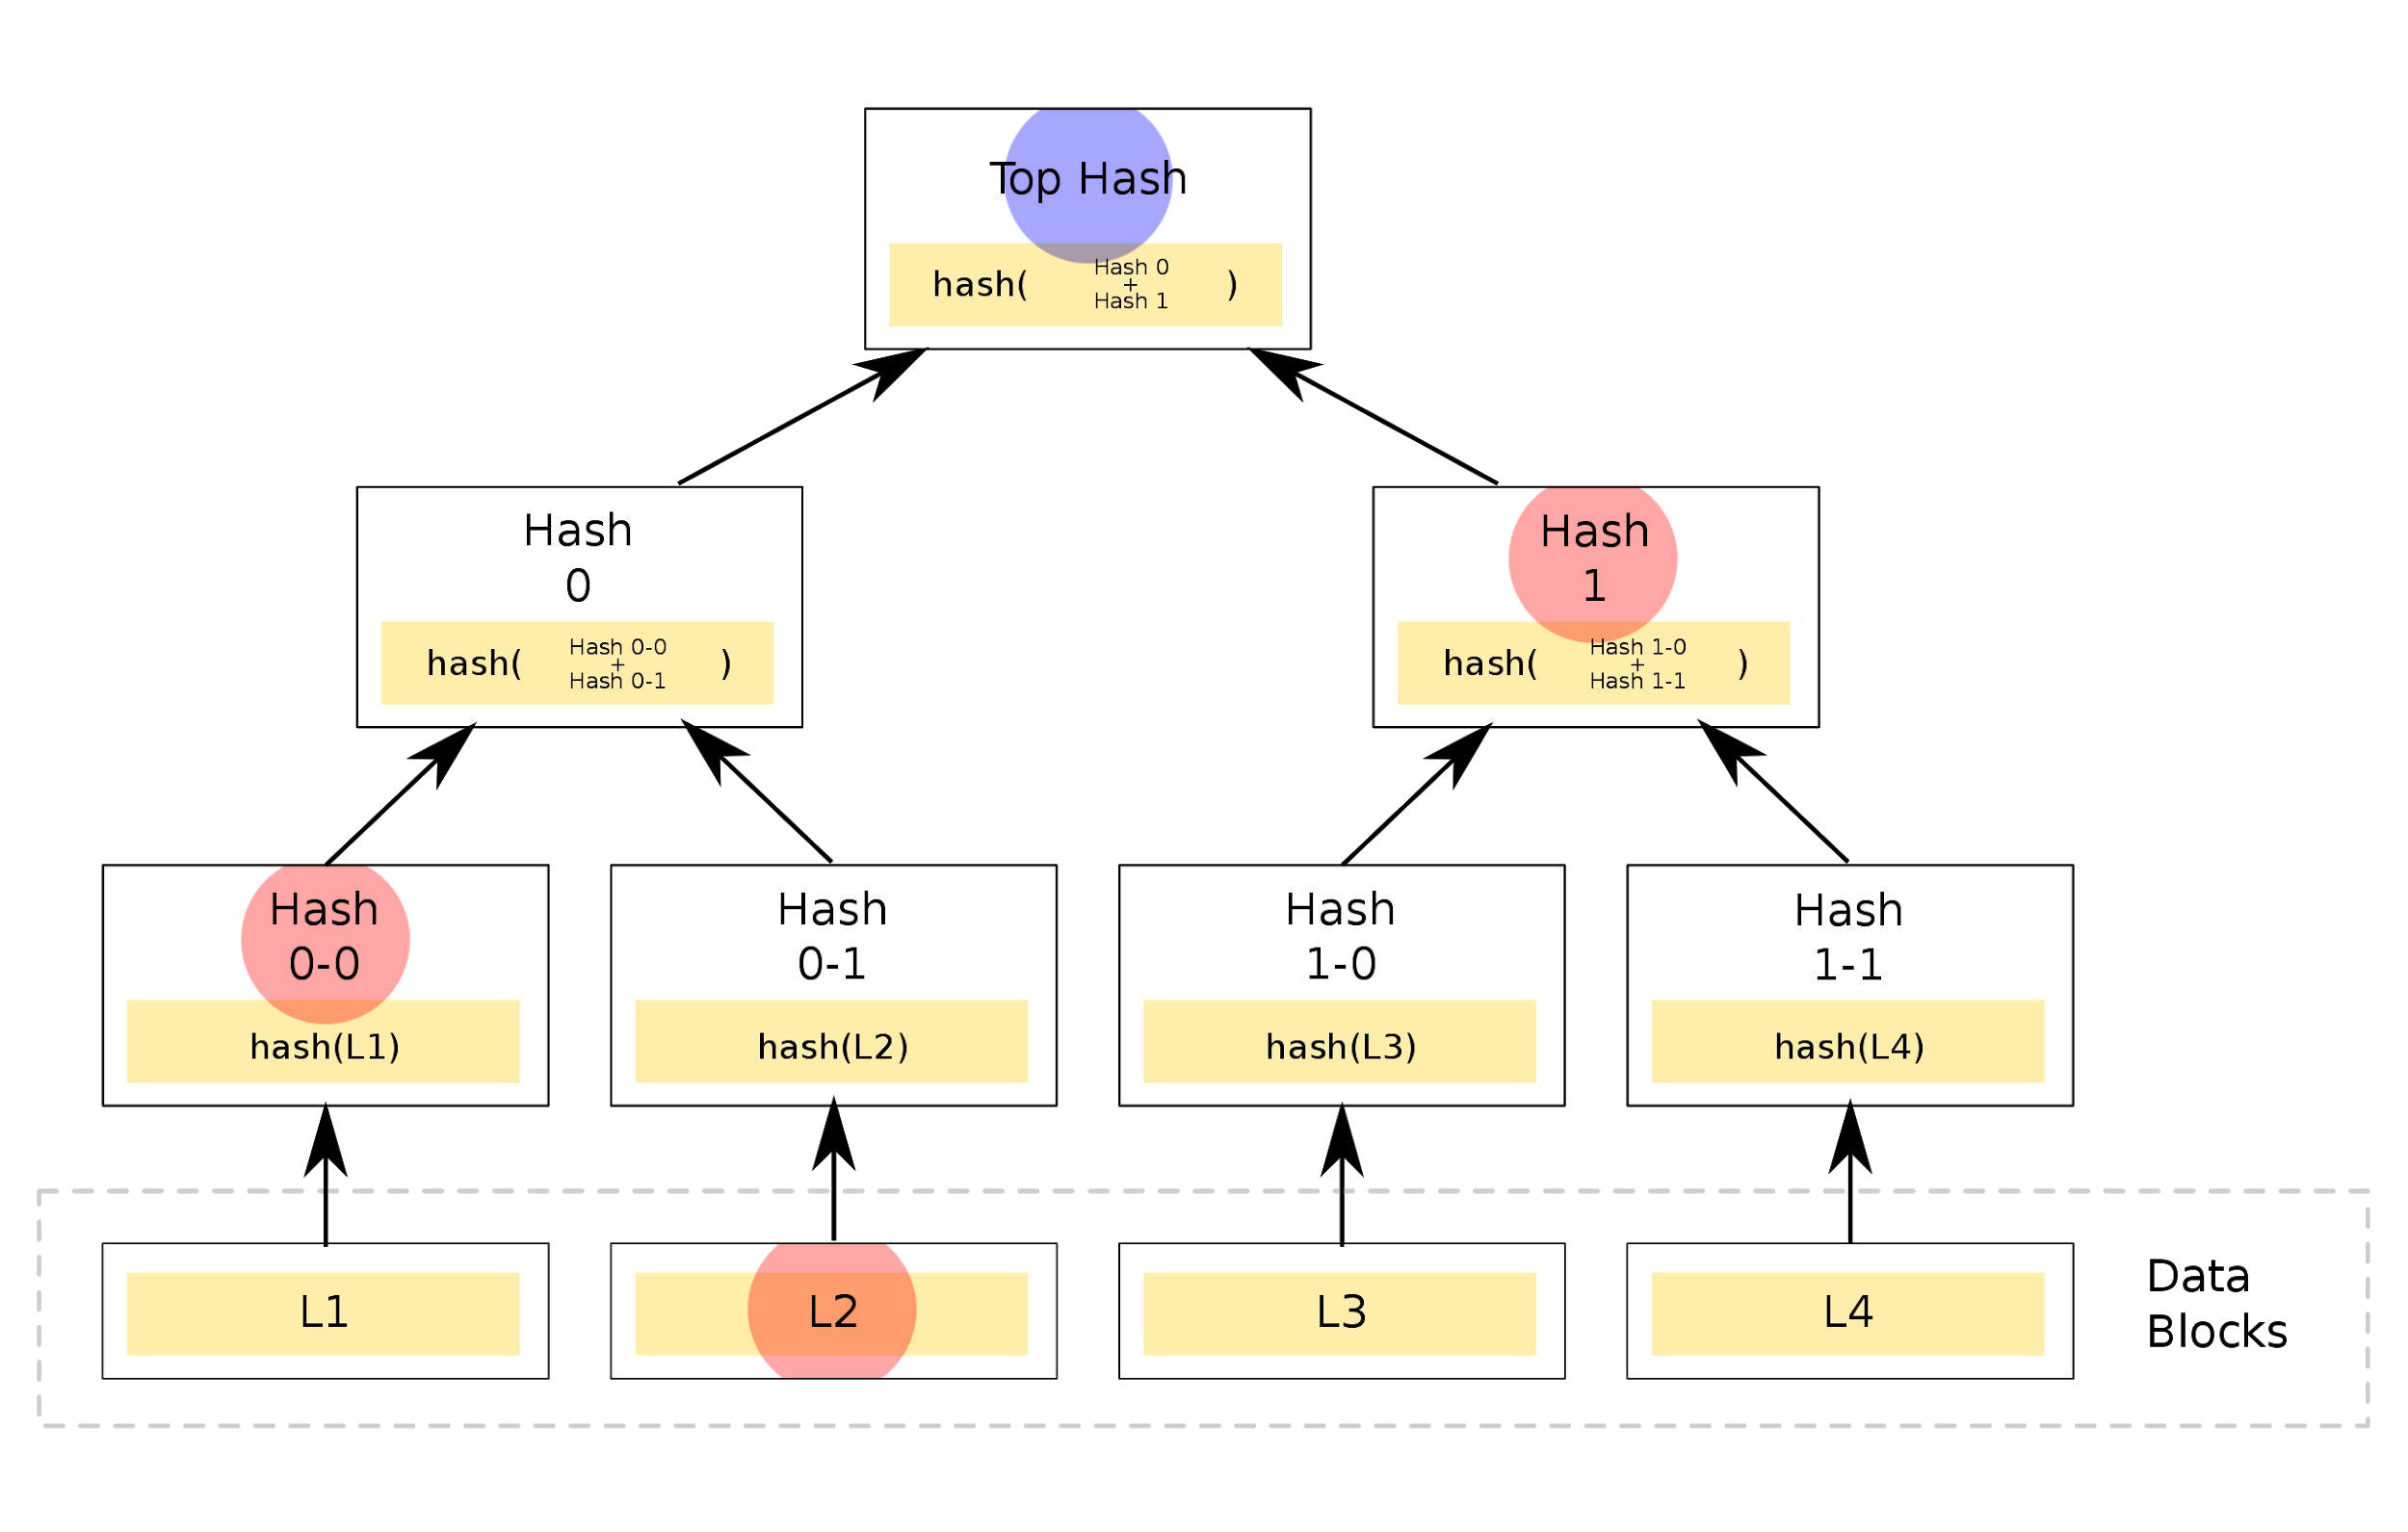
\includegraphics[width=\textwidth]{img/hash-merkle-tree}
    \caption[Merkleho strom pro~hashe]{Merkleho strom pro~veřejné klíče. Je zveřejněn pouze vršek stromu. S~podpisem L2 se zveřejní pouze ty hashe které jsou nutné k~ověření vrcholu (0-0, 1).}
\end{figure}

% TODO Možná ještě Winternitz OTS?


\clearpage
\section{V~souvislosti s~nařízením eIDAS vysvětlete pojmy -- elektronický podpis, zaručený elektronický podpis a kvalifikovaný elektronický podpis, elektronická pečeť, elektronické časové razítko.}
\subsection{Elektronický podpis}
\begin{itemize}
    \item lze tak označit cokoliv, co je použito jako podpis dané osoby a co má elektronikcou podobu
    \item např. napsání našeho jména na~konec mailu
    \item je zřejmé, že není zaručeno jednoznačné spojení s~podepisující osobou
\end{itemize}

\subsection{Zaručený elektronický podpis}
\begin{itemize}
    \item musí být jednoznačně spojen s~podepisující osobou a musí umožňovat její identifikaci
    \item musí být vytvořen pomocí služeb pro~vytváření elektronických podpisů -- pomocí certifikátu (na~ten ale nejsou kladeny žádné požadavky)
    \item nemusí se jednat o~certifikát vydaný kvalifikovaným poskytovatelem, může být jakýkoliv, i~vystavený svépomocí
\end{itemize}

\subsection{Kvalifikovaný elektronický podpis}
\begin{itemize}
    \item zaručený elektronický podpis vytvořený kvalifikovaným prostředkem pro vytváření elektronických podpisů a založen na kvalifikovaném certifikátu pro elektronické podpisy
    \item kvalifikovaný certifikát = vydaný kvalifikovaných poskytovatelem služeb vytvořejícíh důvěru, tzn. poskytovatel, kterému orgán dohledu udělil status kvalifikovaného poskytovatele (v ČR v současnosti 3)
\end{itemize}

\subsection{Elektronická pečeť}
\begin{itemize}
    \item vydává se jen právnických osobám
    \item p. o. nemůže pečetí opatřit cokoliv, ale jen to, čeho je původcem
    \item proces pečetění totožný s podepisováním elektronických podpisem
\end{itemize}

\subsection{Elektronické časové razítko}
\begin{itemize}
    \item elektronický ekvivalent časového určení a místa vlastního podpisu na~listině
    \item elektronický podpis dle znění zákona tento problém neřeší
    \item řeší možné problémy vzniklé odvoláním certifikátu -- byl el. dokument podepsán před odvoláním?
    \item zajišťuje důkaz o~existenci dokumentu v~daném čase
    \item struktura podobná certifikátu, která svazuje kontrolní součet (hash) z~dokumentu s~časem
    \item nutné pro poskytování elektronických notářských služeb a zajištění dlouhodobé archivace elektronicky podepsaných dokumentů
    \item časové razítko je elektronicky podepsáno (vydáváno) autoritou pro vydávání časových razítek -- Time Stamping Authority (TSA)
    \item elektronicky podepsaná struktura čas. razítka:
    \begin{itemize}
        \item jméno vydavatele (jméno TSA)
        \item jedinečné sériové číslo razítka
        \item kontrolní součet (hash) z~dokumentu a čas
    \end{itemize}
\end{itemize}
Požadavky na zdroj času
\begin{itemize}
    \item musí pocházet z oficiálního důvěryhodného zdroje -- např. od~náhodní časové autority
    \item čas nesmí být možné cestou změnit
    \item vždy musí být možné zpětně dosledovat zdroj času, tedy celou hierarchii časových serverů
\end{itemize}
Vydání časového razítka
\begin{itemize}
    \item žádá se prostřednictvím klientské aplikace
    \item klient vytvoří a odešle žádost o časové razítko ve standardizovaném formátu 
    \item žádost je datová struktura obsahující hash z~dokumentu
    \item TSA v~případě kladné odpovědi odesílá odpověď na~žádost obsahující časové razítko
\end{itemize}


\clearpage
\section{Autentizační protokoly -- na~jakém principu pracují, využívané proměnné parametry, hodnocení jejich bezpečnosti (BAN logika).}

\subsection{Princip}
\begin{itemize}
    \item výzva -- odpověď
    \item mezi dvěma entitami nebo s~využitím třetí důvěryhodné strany
    \item ověřují správnost a čerstvost autentizačního požadavku
    \item výzva musí být čerstvá - využívají náhodná čísla, sekvenční čísla nebo časová razítka
\end{itemize}

\subsection{Využívané proměnné parametry}
\begin{itemize}
    \item sekvenční číslo
    \begin{itemize}
        \item tajné, nutné ukládat poslední použité číslo
        \item při každém použití se sekvenční číslo inkrementuje o~1
        \item v~případě desynchronizace je nutné využít nějaký autentizační protokol k~synchronizaci
    \end{itemize}
    \item časové razítko
    \begin{itemize}
        \item využívá se maximálního povoleného zpoždění (acceptance-window) přijaté zprávy
        \item přijatá časová razítka jsou ukládána pro~případ, kdyby útočník chtěl provést útok přehráním v~povoleném časovém okně nebo v~případě změny hodin u~ověřovatele
    \end{itemize}
    \item náhodné číslo použitelné pouze jednou (nonce = number used only once)
    \begin{itemize}
        \item nevyžaduje synchronizaci
        \item ověřovatel ho zašle protstraně a ta jej použije v~autentizační odpovědi
        \item po~použití je vyřazeno z databáze
        \item pokud je nonce dostatečně velký (např. 128~b), tak náhodný výběr snižuje pravděpodobnost výběru stejného nonce na~zanedbatelnou úroveň
    \end{itemize}
\end{itemize}

\subsection{Hodnocení bezpečnosti - BAN logika}
\begin{itemize}
    \item BAN logika -- slouží k~formálnímu popisu bezpečnosti autentizačním protokolů
    \item jedna z~prvních a nejpoužívanějších logik pro~formální ohodnocení autentizačních protokolů, určena pro~kryptografii se sdíleným i~veřejným klíčem
    \item jedná se o~epistemickou a doxastickou logiku (poddruhy modální logiky zabývající se úvahami a znalosti a víře) -- logiky využívané v~PC vědě a umělé inteligenci
    \item zabývá se autentizačními protokoly na~abstrajtní úrovni (neřeší konkrétní implementaci zkoumaného protokolu a problémy s tím spjaté)
\end{itemize}

Otázky BAN logiky
\begin{itemize}
    \item čeho chce zkoumaný protokol dosáhnout?
    \item potřebuje zkoumaný protokol více předpokladů než jiný protokol?
    \item vykonává zkoumaný protokol cokoliv nepotřebného, jenž by mohlo být vypuštěno bez~ohrožení bezpečnosti?
    \item šifruje zkoumaný protokol něco, co by mohlo být zasláno v~otevřené formě bez~ohrožení bezpečnosti? \\
\end{itemize}

Definované konstrukce BAN logiky
\begin{itemize}
    \item P věří X
    \begin{itemize}
        \item účastník P věří výroku X, nebo by měl být oprávněný věřit X
        \item účastník P může jednat, jako by X bylo pravdivé
        \item hlavní konstrukce logiky
    \end{itemize}
    \item P vidí X
    \begin{itemize}
        \item účastník P přijal zprávu obsahujcí výrok X, jenž může přečíst a zopakovat X (např. po dešifrování)
    \end{itemize}
    \item P vyslovil (jednou řekl) X
    \begin{itemize}
        \item účastník P v~určitém čase zaslal zprávu obsahující výrok X. 
        \item není známo, zda-li byla zpráva odeslána před dlouhou dobou nebo v~průběu současného běhu protokolu
        \item je však známo, že účastník P věřil X, když odesílal zprávu \\
    \end{itemize}
    \item pravidlo význam zprávy (message meaning)
    \begin{itemize}
        \item tato pravidla popisují, jakým způsobem lze odvodit důvěry o~původu zpráv
    \end{itemize}
    \item pravidlo ověření aktuálnosti zprávy (nonce verification)
    \begin{itemize}
        \item využívá se ke~kontrole aktuálnosti (novosti) zprávy
        \item příjemce může předpokládat, že odesílatel věří jejímu obsahu a můžeme mu také věřit
        \item zajišťuje ochranu proti útoku přehráním
    \end{itemize}
    \item pravidlo novosti celého výroku
    \begin{itemize}
        \item pokud je část výroku nová (fresh), pak je celý výrok nový
    \end{itemize}
    \item pravidlo jurisdikce (jurisdiction)
    \item pravidla důvěry k množině výroků
\end{itemize}
